\subsection{Legge di Geiger-Nuttal}
Si parte da una prima ossevazione sperimentale: il decadimento $\alpha$ è un decadimento a due corpi:
\begin{itemize}
    \item Energia fissata $E_\alpha\sim Q_\alpha$ questo viene fuori dalla cinematica a due corpi. Visto che la massa della particella $\alpha$ è molto minore della massa del nucleo che sta rinculando, la maggior parte dell'energia cinetica (e quindi della $Q$ viene presa dalla particella $\alpha$);
    \item Si osserva una forte dipendenza di $\lambda$ da $Q$
\end{itemize}
%IMMAGINE geg pot
\begin{figure}[htp!]
  \centering
  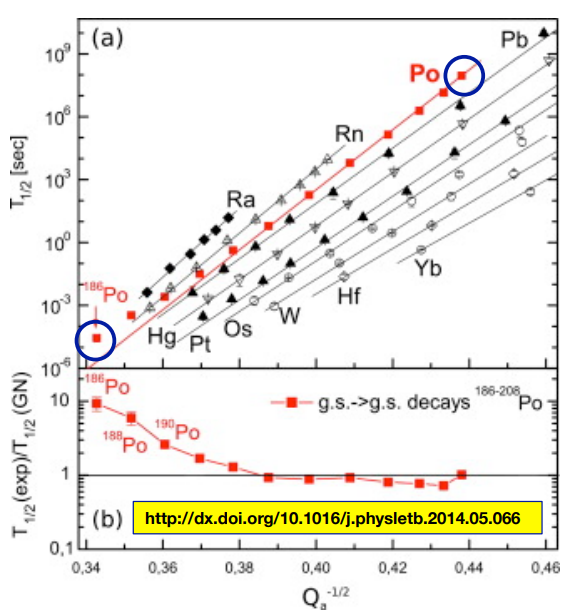
\includegraphics[scale=0.4]{Lezione4/geg.png}
  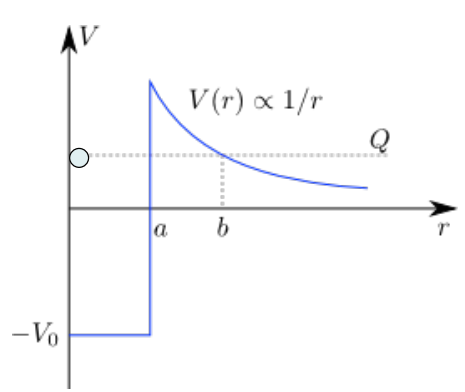
\includegraphics[scale=0.6]{Lezione4/pot.png} 
\end{figure}
Da questo grafico si vede che è una scala lineare in $Q^{-1/2}$. Per quanto riguarda il tempo di dimezzamento varia di parecchi ordini di grandezza. Si nota subito la forte dipendenza.
\begin{equation*}
    \ln{\tau_{1/2}}=a+\frac{b}{\sqrt{Q}}
\end{equation*}
Questa è detta \textbf{Legge di Geiger-Nuttal} ed è empirica. Piccole variazione di energia risultano a grandi differenze nelle costanti di decadimento. Esempio:
\begin{itemize}
    \item $\ch{^{208}Po}$, $Q=5.2\,MeV$, $\tau_{1/2}\sim10^8\,s$
    \item $\ch{^{186}Po}$, $Q=8.6\,MeV$, $\tau_{1/2}\sim10^{-5}\,s$
\end{itemize}
La spiegazione qualitativa di questo comportamento fu proposta da Gamow e vede le cause nell'\textbf{effetto tunnel quantistico}.
\subsection{Modello di Gamow}
La legge di Gaiger-Nuttal può venire spiegata fenomenologicamente dal \textbf{modello di Gamow}: Il nucleo $(A,Z)$ è costituito da una particella $\alpha$, intrappolata nel potenziale generato dal "resto" del nucleo $(A-4,Z-2)$. Il potenziale può essere schematizzato in questa maniera estremamente semplificata. Guardando la prima parte io so che la particella è dentro il nucleo sente delle forze nucleari che sono a breve range, dipende da quanti nucleoni sono vicini a lei e quindi in prima approssimazione posso dire che in quel momento è circa costante. Appena la particella $\alpha$ inizia ad uscire dal nucleo, l'energia di legame diminuisce piano piano ma che in questo modello approssimo come transizione istantanea. Visto che il potenziale dovuto alla interazione nucleare è ora "trascurabile" ciò che rimane è proprio l'interazione coulombiana. 

Questa idealizzazione vale solo all'interno dell'atomo. Questo perchè una volta fuori dall'atomo la particella $\alpha$ non interagisce più in maniera elettrostatica in quanto gli elettroni rendono il tutto neutro.

Guardando sempre lo schema del potenziale, classicamente se la particella $\alpha$ ha un'energia rappresentata dalla linea tratteggiata, sarebbe confinata all'interno del raggio $a$ del nucleo. In meccanica quantistica però ha una probabilità $P$ non nulla di attraversare la barriera per effetto tunnel. Questa rimane comunque un'approssimazione ma ci permette di capire subito gli effetti salienti del fenomeno.  All'interno del nucleo la particella $\alpha$ ha una velocità:
\begin{equation*}
    v=\sqrt{\frac{2(Q+V_0)}{m}}
\end{equation*}
La particela colpisce la barriera con una frequenza $f=v/2a$. \textbf{Il rate di decadimento }è $fP$. Dando un po' di valori: per $V_0=30\,MeV$, $Q=5\,MeV$, $A=200$ abbiamo $v=0.14\,c=0.42\times10^9\,m/s$ e una frequenza $f=3\times10^{21}\,Hz$. Notare che la velcoità è coerente con la trattazione non relativistica. Il numero $f$ è molto elevato e sono un bel po' di tentativi al secondo in cui la particella $\alpha$ tenta di uscire dal nucleo.

La probabilità di superare la barriera di potenziale è data da:
\begin{equation*}
    P=e^{-2G}
\end{equation*}
Dove il fattore $G$ è detto \textbf{fattore di Gamow} ed è definito da un'integrale sulla zona classicamente proibita:
\begin{equation*}
    G=\int_a^b\sqrt{\frac{2m}{\hbar^2}(V(r)-Q)}dr
\end{equation*}
Per fissare le idee, consideriamo il decadimento $\alpha$ del $\ch{^{232}Th}$ ($Z=90$). Con potenziale (coulombiano tra il nucleo risultante):
\begin{equation*}
    V(r)=\frac{(Z-2)2\alpha\hbar c}{r}
\end{equation*}
\begin{itemize}
    \item $a=r_0A^{1/3}=1.2A^{1/3}\,fm=7.4\,fm$
    \item $Q=4.05\,MeV$ (visto che la catena di decadimento in cui il progenitore aveva una vita media più lunga e come ci aspettiamo dalla legge di Gaiger-Nuttal ci aspettiamo un valore molto piccolo)
    \item $V(a)=34.2\,MeV$ si nota che di solito l'interazione forte è più intensa dell'interazione elettromagnetica, tantè che esistono tanti nuclei con un numero elevato di protoni che dal punto di vista elettrostatico vorrebbero uscire. Tuttavia quando abbiamo $Z$ molto grande, abbiamo che il termine repulsivo elettromagnetico è confrontabile con l'interazione forte. Infatti il picco della barriera ha la stessa altezza della buca, siamo sempre intorno sulla trentina di $MeV$.
    \item imponendo che $V(r)=Q$ posso trovare il punto $b$ in cui termina la barriera di potenziale.
\end{itemize}
\begin{equation*}
    b=\frac{(Z-2)2\alpha\hbar c}{Q} =62.5\,fm
\end{equation*}
Quindi vediamo che questo $b$ è molto maggiore rispetto alle dimensioni nucleari.
\subsection{Effetto tunnel}
Un potenziale generico, $V(r)$, può essere visto come sequenza di una serie di barriere infinitesime. Ciascuna ha una probabilità di essere attraversata da:
\begin{equation*}
    P\approx4e^{-2k_0dr}=4\text{exp}\left(-2\sqrt{\frac{2m}{\hbar^2}(V(r)-Q)}dr\right)
\end{equation*}
La probabilità di attraversare la barriera completa è data dal prodotto delle probabilità di attraversare le barriere infinitesimali:
\begin{equation*}
    P\approx4e^{-2\int k_0dr}=4\text{exp}\left(-2\int_a^b\sqrt{\frac{2m}{\hbar^2}(V(r)-Q)}dr\right)
\end{equation*}
Ovvero
\begin{equation*}
    P\approx4e^{-2G} \quad G=\int_a^b\sqrt{\frac{2m}{\hbar^2}(V(r)-Q)}dr
\end{equation*}
con $G$ detto \textbf{Fattore di Gamow}.
\subsection{Fattore di Gamow}
Mettendo insieme i risultati ottenuti otteniamo che la probabilità di decadimento per unità di tempo è data da:
\begin{equation*}
    \lambda=\nu P=\frac{v}{2a}4e^{-2G}=\sqrt{\frac{2(Q+V_0)}{m}}\frac{2}{a}e^{-2G}
\end{equation*}
Ricordiamo che le approssimazioni fatte rendono queste formule applicabili solo per trovare l'ordine di grandezza della vita media. Calcoliamo adesso $G$ per il potenziale di Coulomb.
\begin{equation*}
    b=\frac{(Z-2)2\alpha\hbar c}{Q}
\end{equation*}
Imponendo il potenziale elettrostatico uguale a $Q$ in $b$. Arrivando alla formula finale:
\begin{equation*}
    G=\sqrt{\frac{2mc^2}{Q}}\alpha[2(Z-2)]f\left(\frac{a}{b}\right)
\end{equation*}
dove $f(a/b)$ è definita dalla funzione:
\begin{equation*}
    f\left(\frac{a}{b}\right)=\left[\arccos{\sqrt{\frac{a}{b}}}-\sqrt{\frac{a}{b}-\frac{a^2}{b^2}}\right]
\end{equation*}
La \textbf{vita media} risulta pertando
\begin{equation*}
    \tau=\frac{1}{\lambda}=\sqrt{\frac{m}{2(Q+V_0)}}\frac{a}{2}e^{2G}=\sqrt{\frac{m}{2(Q+V_0)}}\frac{a}{2}\text{exp}\left[ 2\alpha\sqrt{\frac{2mc^2}{Q}}[2(Z-2)] f\left(\frac{a}{b}\right)\right]
\end{equation*}
Vediamo che la formula trovata giusctifica la \textbf{legge di Geiger-Nuttal} una volta fatto il logaritmo:
\begin{equation*}
    \ln{\tau}=\ln{\left( \sqrt{\frac{m}{2(Q+V_0)}}\frac{a}{2} \right)}+2\alpha\sqrt{\frac{2mc^2}{Q}}[2(Z-2)] f\left(\frac{a}{b}\right)
\end{equation*}
Vediamo che c'è una debole dipendenza da $\ln{Q+V_0}$, una dipendenza da $Q^{-1/2}$ e le famiglie di curve in funzioni di $Z$. Se andiamo a confrontare il valore della vita media sperimentale e quello ottenuto dal modello di Gamow si vede che ci da una dipendenza abbastanza simile anche se ci sono alcuni ordini di grandezza. Infatti il modello è corretto per quanto riguarda la dipendenza funzionale, c'è un fattore $100$ tra il modello sperimentale e il modello semplificato. Questo modello sembra grosso anche se bisogna tener conto che rientra nell'esponenziale e quindi anche una piccolissima approssimazione può potare delle importanti conseguenze.

Un'altra cosa importante da notare è che se facessi una semplice considerazione energetica guardando la curva che esprime l'energia di legame per nucleone in funzione del numero di di massa $A$ mi verrebbe da chiedermi: ma perchè i decadimenti non avvengono con il $\ch{^{14}C}$ visto che anche nella sua posizione è presente un picco anche più alto dell'elio-4? La risposta risiede proprio dal termine $2(Z-2)$ che nel caso del carbonio $12$ ci sarebbe il $6$ quindi avrei una barriera di potenziale $3$ più grande e quindi è meno probabile la particella superi la barriera coulombiana (vedi esercizi).
\subsection{Decadimenti alpha}
Il risultato finale è che il nucleo è un oggetto composto, per cui può trovarsi in diversi stati interni. Il decadimento $\alpha$ non è necessario che lasci il nucleo in uno stato di energia minima. Ma possono avvenire su stati eccitati del nucleo figlio.